\documentclass[12pt]{article}
\usepackage[utf8]{inputenc}
\usepackage[upright]{fourier}
\usepackage[T1]{fontenc}
%\usepackage{lmodern}
\usepackage{graphicx}
\usepackage[%
      a4paper,%
      textwidth=16cm,%
      top=2cm,%
      bottom=2cm,%
      headheight=25pt,%
      headsep=12pt,%
      footskip=25pt]{geometry}%
\usepackage[frenchb]{babel}
\title{Manuel Utilisateur :\\Casse-Briques multijoueur}
\author{Groupe 44 \\ Matthias Roger, Jean-Luc Hervy, Jocelyn Bourduge, Mohammed Amine Tourari,\\ Amine Er-roundi, Robin Xambili}
\date{}

\begin{document}

\begin{titlepage}
    \maketitle
    \thispagestyle{empty}
    \tableofcontents
    \pagenumbering{arabic} % pour la numérotation 1, 1.1 ...
\end{titlepage} 


\section{Objectif Général du projet}
	Notre projet consiste à réaliser un jeu de casse-briques permettant de joueur à plusieurs joueurs (en local ou en réseau). Le casse-briques est un jeu d'arcade dont le principe général est de détruire, au moyen d'une ou plusieurs balles, un ensemble de briques se trouvant dans un niveau.


\section{Principe du jeu}
	\subsection{Principe de base}
	Chaque joueur contrôle une barre sur un des bords de la carte de jeu. Cette barre permet de renvoyer les balles qui arrivent dessus. Si une balle traverse le bord d'un joueur, celui-ci perd une vie. Un joueur perd quand il n'a plus de vie. Le but du jeu est d'être le dernier joueur en vie, ou de casser toutes les briques, dans ce cas le joueur avec le score le plus élevé gagne.
	
	\subsection{Mode multijoueur}
	Le mode multijoueur permet de jouer à deux, trois ou quatre joueurs.
	\begin{itemize}
	\item \textbf{Deux joueurs : }face à face, séparés par les briques.\\
	\begin{figure}[!htp]
  			\caption{\label{étiquette} Exemple 2 joueurs}
  			\centerline{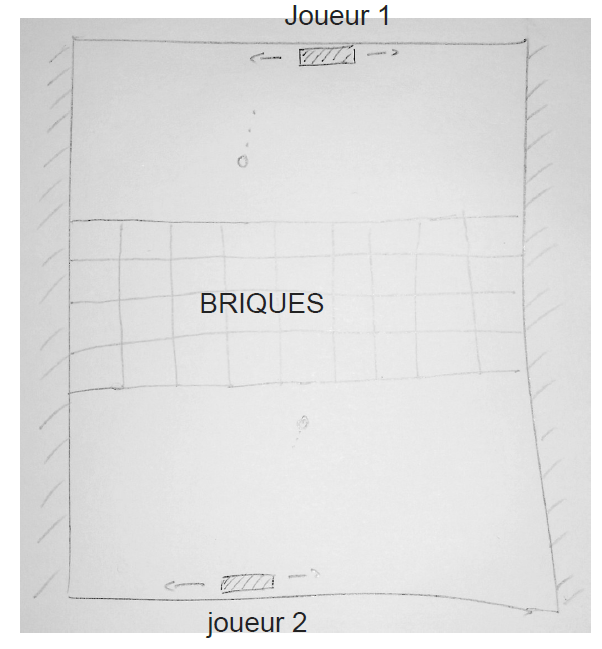
\includegraphics[scale=0.9]{multi_2_joueurs}}
	\end{figure}
	\newpage
	
		
	\item \textbf{Quatre joueurs : }un joueur sur chaque coté, les briques sont rassemblées au centre.\\
	\begin{figure}[!htp]
  			\caption{\label{étiquette} Exemple 4 joueurs}
  			\centerline{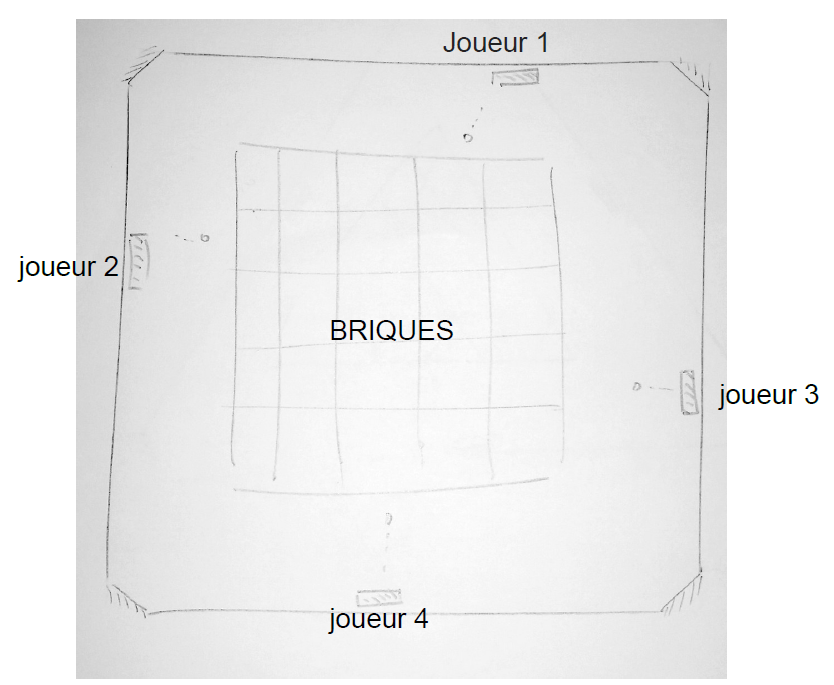
\includegraphics[scale=0.7]{multi_4_joueurs}}
	\end{figure}
	\end{itemize}
	~\\
	
	
\section{Gestion des balles et jouabilité}

La partie commence avec une balle par joueur : une balle est collée sur la barre de chacun des joueurs pendant le décompte de départ à la fin duquelle les balles sont libérées et la partie commence.\\\\
Toutes les balles sont identiques, elles sont jouables par tous les joueurs.\\\\
Certaines briques peuvent mettre en jeu de nouvelles balles, le niveau de difficulté augmente logiquement avec leur nombre. Le fait de commencer avec un grand nombre de vies par joueur permet des parties suffisamment longues et une certaine équité entre les joueurs qui se retrouveront alternativement en situation de difficulté (un grand nombre de balles en jeu peut mettre dans une situation de difficulté un joueur à un moment donné, qui ne pourra pas tout renvoyer et perdra ainsi un grand nombre de vies en peu de temps).\\\\
Le nombre de balles en jeu doit toujours au moins égaler le nombre de joueur encore en vie. Pour cela, lorsque le nombre de balles tombe en dessous du nombre de joueurs, le joueur qui vient de perdre une vie disparait, perd ses bonus, et réapparait avec une nouvelle balle si il lui reste au moins une vie. \\\\Dans le cas ou plusieurs balles sont perdues par un même joueur ou si le joueur n'a plus de vies, les balles manquantes réapparaissent devant les joueur sans balle. Ceci n'arrive que si le nombre minimum de balles en jeu n'est plus atteint.

\section{Types de briques}

	Différents types de briques sont disponibles dans le jeu : 
	\begin{itemize}
		\item \textbf{Brique ordinaire : }ce type de briques représente la brique classique du jeu, qui ne contient aucun bonus et qui se casse du premier contact avec une balle.
		\item \textbf{Brique semi-incassable : }ce type de briques a besoin de plus d'un contact de balle pour ce casser, éventuellement 2 ou plus. 
		\item \textbf{Brique incassable : }ce type de briques apparaît rarement sur le jeu, cette brique ne peut être détruite par les contacts avec les balles, mais elle peut se casser si elle se trouve dans l'entourage d'une brique explosive, en collision avec une balle. Il n'est pas nécessaire de casser ce type de brique pour finir un niveau
		\item \textbf{Brique explosive : }ce type de briques permet de débarrasser la carte de jeu de plusieurs briques de la partie, le nombre de briques détruites dépend du niveau de difficulté.
		\item \textbf{Brique à balles : }cette brique une fois détruite, libère un nombre de balles entre 1 et 3.
	\end{itemize}
		
\section{Cartes de jeu}
		
	\subsection{Cartes prédéfinies, niveaux de difficultés et génération procédurale}
	
	Le joueur peut jouer sur des cartes prédéfinies ou des cartes générées aléatoirement.\\
	

\section{Gestion des scores}

	\subsection{Calcul du score}
	Chaque fois qu'une balle casse une brique, le score du dernier joueur à avoir toucher la balle augmente de 1\\
	
	\newpage

\section{Menu}

	Le menu permet de sélectionner un mode de jeu.\\

	\begin{figure}[!h]
  			\caption{\label{étiquette} Écran Principal}
  			\centerline{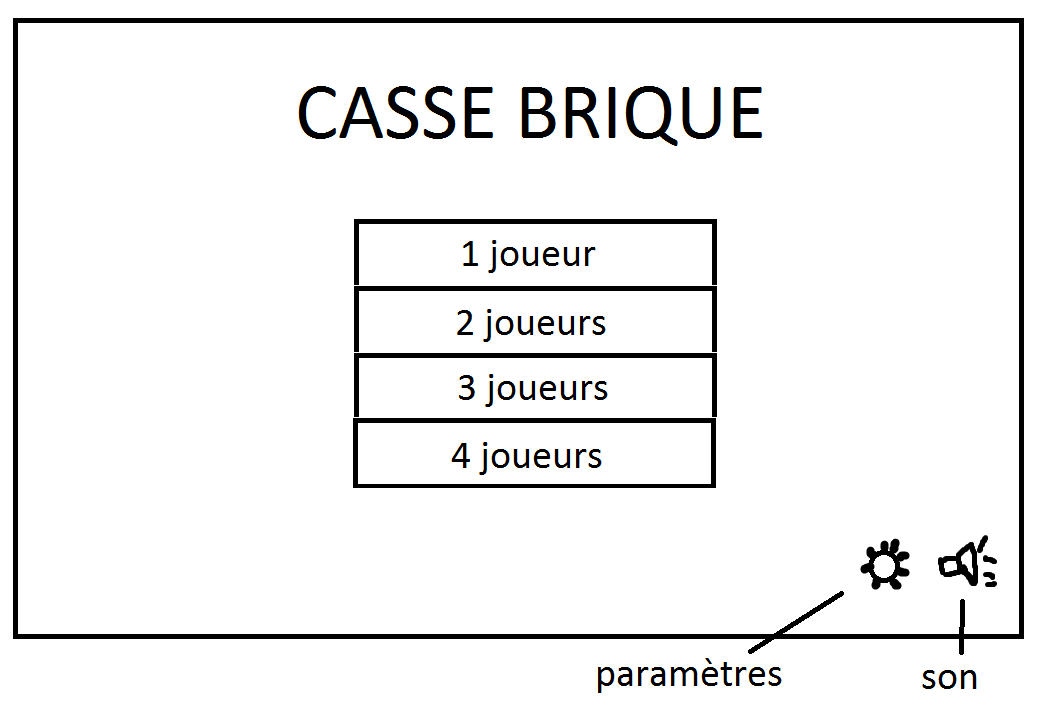
\includegraphics[scale=0.5]{menu}}
	\end{figure}
	
\end{document}
